\let\negmedspace\undefined
\let\negthickspace\undefined
\documentclass[journal]{IEEEtran}
\usepackage[a5paper, margin=10mm, onecolumn]{geometry}
%\usepackage{lmodern} % Ensure lmodern is loaded for pdflatex
\usepackage{tfrupee} % Include tfrupee package

\setlength{\headheight}{1cm} % Set the height of the header box
\setlength{\headsep}{0mm}     % Set the distance between the header box and the top of the text

\usepackage{gvv-book}
\usepackage{gvv}
\usepackage{cite}
\usepackage{amsmath,amssymb,amsfonts,amsthm}
\usepackage{algorithmic}
\usepackage{graphicx}
\usepackage{textcomp}
\usepackage{xcolor}
\usepackage{txfonts}
\usepackage{listings}
\usepackage{enumitem}
\usepackage{mathtools}
\usepackage{gensymb}
\usepackage{comment}
\usepackage[breaklinks=true]{hyperref}
\usepackage{tkz-euclide} 
\usepackage{listings}
% \usepackage{gvv}                                        
\def\inputGnumericTable{}                                 
\usepackage[latin1]{inputenc}                                
\usepackage{color}                                            
\usepackage{array}                                            
\usepackage{longtable}                                       
\usepackage{calc}                                             
\usepackage{multirow}                                         
\usepackage{hhline}                                           
\usepackage{ifthen}                                           
\usepackage{lscape}
\usepackage{tikz}
\usetikzlibrary{patterns}
\begin{document}


\bibliographystyle{IEEEtran}
\vspace{3cm}


\numberwithin{equation}{enumi}
\numberwithin{figure}{enumi}
\renewcommand{\thetable}{\theenumi}


% Marks the beginning of the document

\bibliographystyle{IEEEtran}
\vspace{3cm}


\title{1.2.10}
\author{AI25BTECH11004-B.JASWANTH}
% \maketitle
% \newpage
% \bigskip
{\let\newpage\relax\maketitle}


\renewcommand{\thefigure}{\theenumi}
\renewcommand{\thetable}{\theenumi}
\setlength{\intextsep}{10pt} % Space between text and floats

\textbf{Question}\\
Find the vector joining the points $\Vec{P}$(2,3,0) and $\Vec{Q}$(-1,-2,-4) directed from $\vec{P}$  to $\vec{Q}$. \\
\textbf{Solution}: \\
\begin{table}[h!]
	\centering
	

	\caption{variables used}
	\label{}
\end{table}\\
 \text{The vector joining $\vec{P}$ and $\vec{Q}$ = $\vec{Q}$ - $\vec{P}$}\\
    $\implies$ $\vec{Q}-\vec{P}$ = \myvec{-1\\-2\\-4} - \myvec{2\\3\\0} = \myvec{-3\\-5\\-4} \\
    $\implies$ The desired vector is \myvec{-3\\-5\\-4} 
 
\begin{figure}[h!]
 \centering
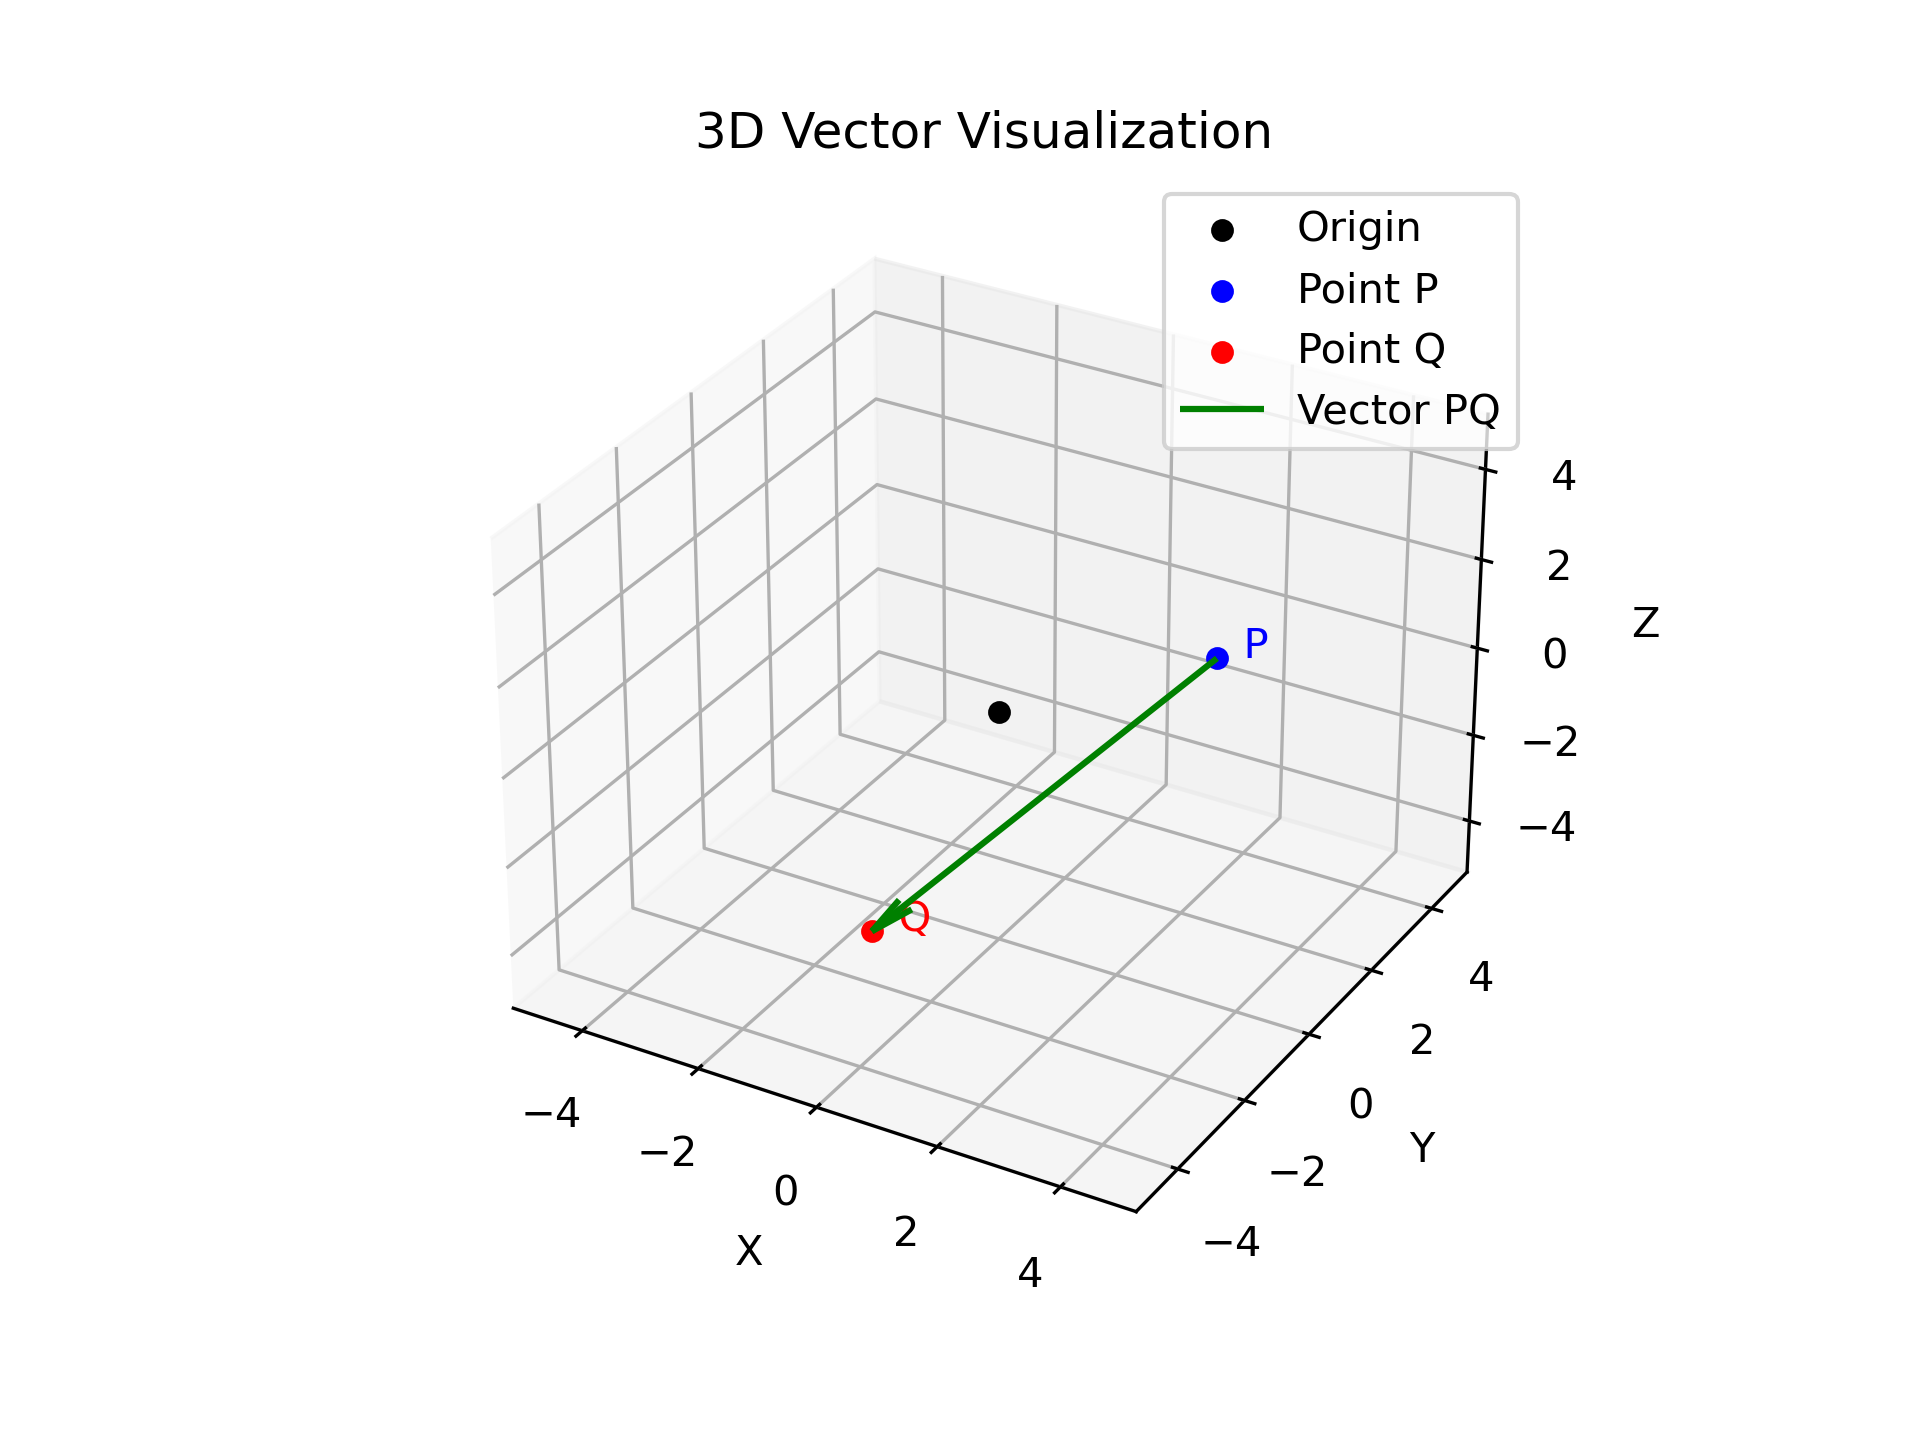
\includegraphics[width=0.7\linewidth]{figs/01.png}
\caption{Line segment represent the vector}
\label{stemplot}
\end{figure}







\end{document}
